\chapter{Speichersysteme in Videospielen}\label{ch:videospiele}
In diesem Kapitel wird die Praxis von Speicher- und Ladesystemen betrachtet. Dabei werden verschiedene Spiele analysiert, um deren Prozesse des Speicherns und Ladens des Spielstandes genauer zu verstehen. Als erstes wird das Sandbox-Spiel Minecraft und danach das Strategiespiel Factorio angeschaut. 
%--------------------------------------------------------------------------


%--------------------------------------------------------------------------
\section{Minecraft}
Minecraft ist ein Sandbox-Spiel\footnote{Ein Sandbox-Spiel lässt Spieler frei entscheiden, was mit der Spielwelt gemacht werden soll. Es gibt keine feste Geschichte im Spiel, die verfolgt werden muss.\cite{ocio2009multi}}, welches von Mojang Studio entwwickelt wurde. Minecraft gilt unter den meistverkauften Videospiele aller Zeiten und kann auf eine Vielzahl von Plattformen gespielt werden.\cite{ignBestSellingVideo} Es wird in einer dreidimensionalen Welt, die aus Blöcken besteht, gespielt und es kann mit Entitäten interagiert werden. Es gibt verschiedene Spielmodi, wie zum Beispiel ein Überlebens- und Kreativmodus. Beim Überlebensmodus geht es hauptsächlich um das Überleben in der Spielwelt, jedoch kann der Spieler frei entscheiden, was er in der Spielwelt machen wird.\cite{minecraftWikiHome}

In diesem Abschnitt dieser Arbeit wird das Speicher- und Ladesystem von Minecraft genauer betrachtet. Als erstes wird ausgearbeitet, aus welchen Spielobjekten die Welt in Minecraft besteht, um herauszufinden, welche verschiedenen Daten gespeichert werden müssen. Danach wird geschaut, wie diese Daten bei Minecraft aufgeteilt werden, damit nur mit einer Teilmenge der ganzen Daten gearbeitet werden muss. Anschließend wird die Ordnerstruktur einer Spielwelt angeschaut, um ein tieferes Verständnis für die Aufteilung der Daten zu sichern. Danach werden die Formate der Dateien genauer betrachtet, um zu verstehen, wie die einzelnen Daten letztendlich in den Speicher geschrieben werden. Zum Schluss wird angeschaut, wie der Ablauf des gesamten Speicherprozess ist. Es wird erklärt, zu welchen Zeitpunkten der Spielzustand gesichert wird, damit möglichst wenig Daten der Spielwelt verloren gehen. Dabei wurde als Quelle ausschließlich die Minecraft Wiki\footnote{ Minecraft Wiki: \url{https://minecraft.fandom.com/wiki/Minecraft_Wiki}} verwendet, die von dem Minecraft Support empfohlen wurde (siehe die Abbildung \ref{fig:minecraftMail}). Sie dokumentiert alle Daten zu Minecraft, um ein tieferes Verständnis für das Spiel aufzubauen. Dadurch, dass es für Minecraft auch Modifikationen gibt, die von jeglichen Entwicklern geschrieben werden können, gibt es auch Möglichkeiten an den Quelltext von Minecraft zu kommen. Aus rechtlichen Gründen ist es jedoch leider nicht möglich, diesen freizugeben. Viele Inhalte der Minecraft Wiki wurden jedoch noch einmal geprüft, durch analysieren des Quellcodes.\todo{Autor mit einbeziehen; Ich habe den Quellcode mir angeschaut für die Arbeit}



\subsection{Daten}
Bevor sich das Speicher- und Ladesystem von Minecraft genauer angeschaut werden kann, ist es erstmal wichtig zu wissen, mit welchen Arten von Daten Minecraft arbeitet. Die Spielwelt in Minecraft besteht aus verschiedenen Blöcken, Entitäten\todo{Entitäten vs Entitys} und Items. 

\textit{Blöcke} werden in Minecraft nicht einzeln behandelt, sondern als Section, ein Bereich von 16x16x16-Block, gespeichert. Mehr zu dieser Aufteilung bei Minecraft gibt es im Abschnitt \ref{ssec:datenaufteilung}. Informationen, die zu so einem Block gehören, sind die Position, BlockID, Block Zustände und Informationen zum Licht. Die Position eines Blocks wird in der Reihenfolge y-, z- und x-Koordinate gespeichert, für bessere Komprimierung. Jeder Blocktyp hat eine eigene BlockID, die diesen Block genau identifiziert. Der Zustand eines Blocks wird für jede Section in einer Liste namens "BlockStates" abgespeichert. Informationen dessen Zustands können zum Beispiel sein, in welcher Himmelsrichtung der Block plaziert wurde, welche Rotation der Block hat und ob der Block am brennen ist. Welche Zustände ein Block haben kann, hängt auch von dem Blocktyp ab.\cite{minecraftBlockStates} Bei den Informationen zum Licht jedes Blocks gibt es für jede Section zwei Listen namens "BlockLight" und "SkyLight". "BlockLight" speichert wieviel Licht jeder Block ausstrahlt und "SkyLight" wieviel jeder Block an Licht abbekommt. Zusätlich gibt es noch sogenannte Block Entitys, die aber nichts mit den Entitäten des Spieles zu tun haben. Diese Speichern zusätliche Informationen zu einem Block, die in der "BlockStates"-Liste nicht gespeichert werden konnten.\cite{minecraftChunkFormat}
%Weitere Quelle: ChunkSerializer.java:write()

Eine Entität kann ein Spieler, ein Tier oder Monster sein. Die wichtigste Information einer Entität ist die Position, Geschwindigkeit und Rotation dieser. Des weiteren gibt es viele weitere Informationen zu einer Entität, wie die Luft die die Entität noch übrig hat zum Überleben, die Distanz die eine Entität schon gefallen ist oder wie lange eine Entität noch brennen wird.\cite{minecraftEntityFormat}
%Weitere Quelle: Entity.java:writeWithoutTypeID()

\textit{Items} bei Minecraft existieren im Inventar, in Kisten, in Item Frames oder in Armor Stands\todo{Englisch}. Wenn ein Spieler ein Item fallen lässt, dann werden diese als Entitäten in die Welt platziert und als solche gespeichert. Manche Items können in die Welt platziert werden und werden dann zu neuen Blöcken oder Entitäten. Jedes Item hat die Information "Count", "Slot", "id" und "tag". "Count" und "Slot" definieren, wieviele Items in welchem Inventarplatz liegen. Jedes Item hat dabei eine eigene Identifikationsnummer, mit der diese gespeichert werden. "tag" gibt noch zusätliche Informationen über ein Item, wie die Haltbarkeit oder ob ein Item unzerbrechlich ist.
\cite{minecraftPlayerdatFormat}
\cite{minecraftItem}

%Item werdeb z.B. in player.dat gespeichert



\subsection{Datenaufteilung} \label{ssec:datenaufteilung}
Die Spielwelt von Minecraft, mit seinen Blöcken, Entitäten und Items, werden nach einem Chunk-basiertem System aufgeteilt. Dieses System unterteilt die Welt in verschiedene Gruppierungen und Untergruppen, wobei die oberste Ebene die "Welt" selbst ist. In Minecraft bezeichnet eine "Welt" die Spielwelt, die von einem Spieler erstellt werden kann, und diese Welt wird wiederum in die drei Dimensionen "Overworld", "Nether" und "End" unterteilt.\cite{minecraftWorld}

Jede Dimension bekommt seine eigenen Dateien zum Speichern der Daten (siehe \ref{ssec:ordnerstruktur}). Eine Dimension kann theoretisch aus unendlich vielen Blöcken, Entitäten und Items bestehen. Sie wird dabei auf mehrere Regionen aufgeteilt. Eine Region besteht aus 1024 Chunks, wobei sie 32 Chunks breit und 32 Chunks lang ist.\cite{minecraftRegionFile} 

Was die Größe eines Chunks betrifft, so ist sie statisch und beträgt 16 Blöcke in der Länge, 16 Blöcke in der Breite und die Höhe variiert je nach der jeweiligen Höhe der Welt. Seit der Einführung der Minecraft Version 1.18 beträgt die maximale Höhe der Spielwelt 384 Blöcke.\cite{minecraftNewestJavaEdition}\cite{minecraftNewestBedrockEdition} Um diese Struktur weiter zu verfeinern, wird jeder Chunk in Sektionen unterteilt. Eine Sektion besteht aus insgesamt 4096 Blöcken, was bedeutet, dass sie 16 Blöcke in der Länge, Breite und Höhe umfasst.\cite{minecraftChunk}

%Chunk.java:sections



\subsection{Ordnerstruktur} \label{ssec:ordnerstruktur}
Ein Spieler kann in Minecraft verschiedene Spielwelten erstellen. Dabei bekommt jede dieser Spielwelten einen eigenen Ordner. Wie so ein Ordner aufgebaut ist, ist in der Ordnerstruktur aus \ref{lst:ordnerStrukturMinecraft} zu sehen. Die nicht-markierten Knoten entsprechen einem Ordner und die blauen Knoten sind Dateien in dem Speichersystem. In dem Ordner einer Welt sind noch ein paar weitere Ordner und Dateien, diese sind aber nicht relevant für diese Arbeit. Die erste Datei in dem Ordner, die "level.dat"-Datei, speichert globale Daten über die Spielwelt ab. In den Ordnern "playerdata", "stats" und "advancements" werden Spielerinformationen abgespeichert, über eine "<uuid>.dat"- oder "<uuid>.json"-Datei. Die "uuid" wird dabei durch die Identifikationsnummer des Spielers ersetzt. Wenn alleine gespielt wird, werden viele Spielerdaten auch in der "level.dat"-Datei gespeichert. In dem "stats"- und "advancements"-Ordner werden Statistiken und Fortschritte von jedem Spieler der Welt gespeichert. Falls eine Welt im Mehrspielermodus gespielt wird, enthalten die Dateien im "playerdata"-Ordner alle restlichen Informationen eines Spielers.\cite{minecraftPlayerdatFormat}. Die restlichen Ordner und Dateien speichern den Zustand der Spielwelt. Bei Minecraft gibt es zum Beispiel Weltkarten, die Teile der Spielwelt anzeigen können. Jede Weltkarte kann dabei unterschiedliche bereiche der Welt anzeigen, deshalb gibt es für jede Weltkarte eine "map\_<\#>.dat"-Datei, die den Zustand einer Weltkarte speichert. Die "villages.dat"-Datei speichert die Zustände aller Dörfer der Spielwelt, denn jedes Dorf ist ein komplexes System aus verschiedenen zufällig generierten Entitäten und Gebäuden. Da die Spielwelt von Minecraft aus verschiedenen Dimensionen, namens "Overworld", "Nether" und "End" besteht, werden manche Daten auf verschiedenen Ordnern verteilt. Im "DIM-1"-Ordner werden Informationen zu der "Nether"-Dimension gespeichert und der "DIM1"-Ordner ist für die "End"-Dimension. Die "entities"- und "region"-Ordner zum Beispiel enthalten Informationen über die Entitäten und Regionen der Spielwelt und sind auch in den Ordnern der verschiedenen Dimensionen zu finden. Alle Entitäten und Regionen, die in keinem "DIM-1"- oder "DIM1"-Ordner gespeichert wurden, gehören zu der "Overworld"-Dimension.\cite{minecraftFolderStruc}

\begin{listing}[htp]
    \dirtree{%
    .1 world.
        .2 \textcolor{blue}{level.dat}.
        .2 playerdata.
            .3 \textcolor{blue}{<uuid>.dat}.
        .2 stats.
            .3 \textcolor{blue}{<uuid>.json}.
        .2 advancements.
            .3 \textcolor{blue}{<uuid>.json}.
        .2 data.
            .3 \textcolor{blue}{idcounts.dat}.
            .3 \textcolor{blue}{map\_<\#>.dat}.
            .3 \textcolor{blue}{villages.dat}.
            .3 \dots.
        .2 entities.
        .2 region. 
            .3 \textcolor{blue}{r.<\#>.<\#>.mca}.
        .2 DIM-1.
            .3 entities.
            .3 region.
                .4 \textcolor{blue}{r.<\#>.<\#>.mca}.
            .3 \dots.
        .2 DIM1.
            .3 entities.
            .3 region.
                .4 \textcolor{blue}{r.<\#>.<\#>.mca}.
            .3 \dots.
        .2 \dots.
    } 
    \caption{Ordnerstruktur einer Spielwelt in Minecraft\cite{minecraftFolderStruc}}
    \label{lst:ordnerStrukturMinecraft}
\end{listing}



\subsection{Speicherformate}
Wie schon im vorherigen Abschnitt zu sehen ist, besitzt Minecraft eine handvoll verschiedener Formate, zum Speichern der Daten. Die Dateien haben Formate wie "dat", "mca" und "json". Natürlich existieren auch noch weitere Formate, wie PNG-Dateien für Texturen, da diese Dateien zu den statischen Daten dazugehören, werden diese nicht weiter betrachtet.   

Das DAT-Format wird für jegliche Arten von Informationen verwendet, sei es Video, Audio, PDF oder jede andere Art von Daten. Ein Programm kann DAT-Dateien erstellen und spezifisch für dieses Programm Daten abspeichern und lesen. Für andere Programme sind diese Daten nicht sonderlich hilfreich, da sie für ein spezifisches Programm erstellt wurden.\cite{adobeWhatDAT} Dieses Format wird zum Beispiel für die globalen Spielwelt Informationen in der "level.dat"-Datei oder für Spielerdaten in "<player>.dat"-Dateien, falls die Spielwelt auf einem Server gehosted wird (siehe \ref{ssec:ordnerstruktur}).\cite{minecraftPlayerdatFormat}\cite{minecraftFolderStruc}. 
Die Daten werden dabei im eigenen Format namens \ac{nbt} in diese Dateien geschrieben. Diese Format ist ähnlich zu dem \ac{json}-Format, denn die Daten werden auch hier im Schlüssel-Wert-Prinzip behandelt. Das \ac{nbt}-Format bietet eine Vielzahl an Datentypen, wie Byte, Boolean, verschiedene Zahlen Datentypen, String, List, Compound und Array. Der List-Datentyp ist zum Speichern von mehreren Werten, ohne Schlüssel. Compound ist eine geordnete Liste von Schlüssel-Wert-Paaren. Nachträglich werden in den meisten Fällen die \ac{nbt}-Dateien mit GZip komprimiert.
\cite{minecraftNBT}

\ac{mca} ist ein Dateiformat, zum Speichern von Chunk-Daten. Dabei wird in einer Datei eine Region, also eine Gebiet aus 32x32 Chunks, gespeichert. Jede Datei bekommt dann den Namen "r.<x>.<z>.mca", wobei x und z mit den x und z Koordinaten der Region ersetzt wird. Falls die Koordinaten einer Region gesucht werden, in der ein Chunk drin ist, müssen die Chunk-Koordinaten durch 32 geteilt und abgerundet werden. Eine \ac{mca}-Datei fängt mit einem 8 KiB Header an, der in zwei 4 KiB Blöcken unterteilt ist. Der erste Block beschreibt die Position der Chunks in der Region und der zweite Block speichert die Zeit, wann jeder Chunk zuletzt aktualisiert wurde. Nach dem Header werden alle Zustände der Chunks einer Region gespeichert. Dabei wird für jeden Chunk erst die Länge der Daten in Bytes angegeben, dann die Art der Komprimierung und anschließend die komprimierten Daten.\cite{minecraftRegionFile}\cite{minecraftAnvilFile} Auch in diesen Dateien werden die Daten im \ac{nbt}-Format in komprimiert Form gespeichert.\cite{minecraftNBT}

Das \ac{json}-Format wird für das Speichern von Texten und kleineren Daten verwendet. In Minecraft gibt es Bücher, Schilder und Labels, die der Spieler beschriften und mit Text füllen kann. Bücher zum Beispiel werden dann zwar im \ac{nbt}-Format in den Dateien zu den Spielerdaten gespeichert, aber die Seiten der Bücher werden als serialisierten \ac{json}-Text gespeichert.\cite{minecraftPlayerdatFormat} Die "advancements"- und "stats"-Ordner, die im Abschnitt \ref{ssec:ordnerstruktur} vorgestellt wurden, speichern die Fortschritte der einzelnen Spieler auch im \ac{json}-Format ab. Ansonsten wird \ac{json} hauptsächlich für statische Daten, wie das Verhalten von Entitäten, Blöcken und Items oder Anleitungen für das Bauen von Spielgegenständen.\cite{minecraftJSON}

%Siehe auch: RegionFileCache.java:loadFile(), SaveFormat.java:convertRegions()

\subsection{Speichervorgänge}
In den vorherigen Abschnitten wurde detailliert erörtert, welche Daten in Minecraft gespeichert werden und in welcher Form dies geschieht. Nun stellt sich die Frage nach dem genauen Ablauf des gesamten Speicherprozesses und den Zeitpunkten, zu denen die Daten gesichert werden.

Der Spielzustand einer Welt in Minecraft wird zu verschiedenen Zeitpunkten im Spielverlauf gesichert. Zunächst wird der initiale Zustand der Spielwelt gespeichert, wenn eine Welt neu generiert wird. Doch darüber hinaus erfolgen während das Spiel gespielt wird sowohl automatische als auch manuelle Speicherprozesse.\cite{minecraftSpielstandSpeicherung}

Manuelle Speicherungen finden statt, wenn der Spieler die Pause-Taste betätigt, die in Minecraft der "Esc"-Taste entspricht. Damit hat der Spieler die Möglichkeit, den aktuellen Zustand seiner Welt bewusst zu sichern.\cite{minecraftSpielstandSpeicherung} 

Automatische Speicherungen erfolgen hingegen in regelmäßigen Intervallen. Der Spielzustand wird alle fünf Minuten automatisch gesichert, um sicherzustellen, dass selbst bei unvorhergesehenen Ereignissen oder einem möglichen Absturz des Spiels nur minimaler Fortschritt verloren geht.\cite{minecraftSpielstandSpeicherung}

Chunks die zu weit weg von dem Spieler sind, werden bei Minecraft entladen, da es sehr viele Ressourcen brauchen würde, alle Chunks geladen zu lassen, auch wenn sie nicht aktiv verwendet werden. Bevor diese entladen werden, wird der Zustand des Chunks automatisch gesichert. Dies gewährleistet, dass keine relevanten Chunk-Informationen verloren gehen und diese bei Bedarf wiederhergestellt werden können.\cite{minecraftSpielstandSpeicherung}

Insgesamt sorgen diese verschiedenen Speichermechanismen in Minecraft dafür, dass der Spielverlauf zuverlässig und in verschiedenen Situationen gesichert wird, um den Verlust von Fortschritt auf ein Minimum zu reduzieren.

%Siehe auch: Minecraft.java:createWorld()
%Siehe auch: IntegratedServer.java:tick()



\subsection{Ladevorgänge}



\subsection{Fazit}
\begin{itemize}
    \item Chunk System mit fester Größe, da Limit an Elementen pro Chunk?
    \item Erwähnen, dass beim Spielen die Speicher- und die Ladezeiten nicht auffallen. Zu Beginn sind die Ladezeiten auch gering
\end{itemize}

\todo{Irgendwie zusammenfassen, welche Strategien Minecraft verwendet?}
%--------------------------------------------------------------------------



%--------------------------------------------------------------------------
\section{Factorio}
Factorio ist ein Spiel, wo das Hauptziel ist, eine Fabrik aufzubauen. Als Spieler muss man sich um Ressourcen kümmern, die abgebaut werden müssen, um damit neue Technologien zu erforschen und eine Infrastruktur aufzubauen. Um eine möglichst große Ausbeute für die eigene Fabrik zu erreichen, kann die Produktion automatisiert werden. Im Spiel gibt es außerdem noch Einheimische, die die Ausbeutung der Ressourcen anhalten wollen. Deshalb muss der Spieler zusätzlich zu dem Aufbauen seiner Fabrik diese auch noch vor den Einheimischen verteidigen, damit sie nicht kaputt geht. Factorio wurde von Wube Software in C++ geschrieben und 2016 auf der Plattform "Steam" veröffentlicht. Mittlerweile kann Factorio auf Windows, macOS, Linux und der Nintendo Switch gespielt werden.\cite{factorioMain}\cite{factorioPressFactorio}

In diesem Abschnitt wird das Speicher- und Ladesystem von Factorio genauer betrachtet. Als erstes wird analysiert, welche Daten das Spiel beinhaltet, und wie diese aufgeteilt werden. Anschließend werden die einzelnen Vorgänge des gesamten Speicher- und Ladeprozess angeschaut. Als Bezugsquelle für die Informationen zu dem System von Factorio wurde hauptsächlich mit den Quellen gearbeitet, die Wube Software empfohlen hat (siehe Abbildung \ref{fig:factorioMail}). Für ein tieferes Verständnis über die Prozesse des Spieles wurde außerdem die offiziellen Wiki von Factorio\footnote{Offizielle Wiki von Factorio: \url{https://wiki.factorio.com/} \cite{factorioPressFactorio}} verwendet.

\subsection{Daten}
Factorio benutzt Serialisierung und Deserialisierung, verwendet dabei aber verschiedene Formate zum Speichern der Daten. Welche verschiedenen Arten von Daten dann das Spiel hat, zeigt die Abbildung \ref{fig:factorioSaveStatistic}. Das Kreisdiagramm zeigt welche Arten von Daten wie viel Speicherplatz benötigen, bei 40 MB unkomprimierten Daten. Ungefähr 70\% des Speicherplatzes verbrauchen drei Kategorien der Spielobjekte, die Dekorations-Objekte, Tiles und Entitäten. Tiles sind Rechtecke, die das kleinste Stück in der Spielwelt darstellen. Die Tiles sind auch die Maßeinheiten für alle Gebiets- und Distanzabmessungen. Die Größe von Entitäten wird auch in Tiles angegeben. Zum Beispiel ist das "Rocket Silo", die größte Entität in dem Spiel, neun Tiles breit und lang. Die Spielwelt hat eine maximale Größe von zwei Millionen Tiles in der Breite und Länge, also vier Trillionen Tiles.\cite{factorioMapStructure} Die restlichen Daten sind aus der Blueprint Bibliothek, Physikalische Kräfte, Transportbänder, Oberfläche und Chunk Daten und weiteren kleineren Daten.\cite{factorioFridayFacts270} Die Blueprint Bibliothek ist ein virtuelles Inventar, welche Blueprint-artige Items speichert.\cite{factorioBlueprintLibrary} Ein Blueprint ist zum Duplizieren von Fabrikbereichen. Diese können als Blueprint gespeichert und in der Spielwelt dann eingefügt werden.\cite{factorioBlueprint}. Da ein Spieler eine Vielzahl an Blueprints erstellen kann, müssen diese beim Speicherprozess mit einbezogen werden. Transportbänder sind wichtig zum maximieren der Produktion und Automatisierung dieser. Sie transportieren die abgebauten oder hergestellten Ressourcen. Was genau in einem Chunk drin ist, ist in dem Abschnitt \ref{ssec:factorioDatenaufteilung} zu sehen. 

\begin{figure}[htp]
    \centering
    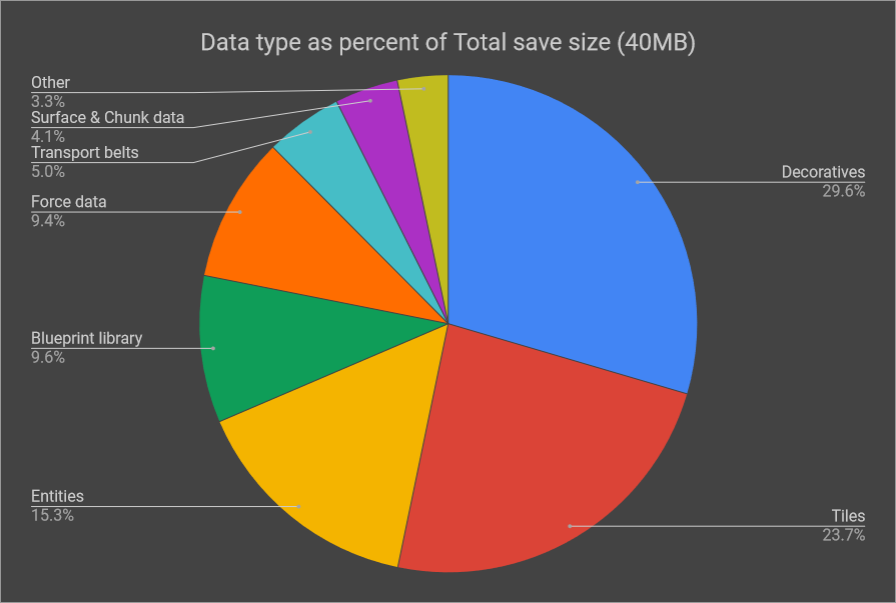
\includegraphics[width=0.9\textwidth]{images/factorio_save_statistic.png}
    \caption{Anteil der Datentypen beim Speichern\cite{factorioFridayFacts270}}
    \label{fig:factorioSaveStatistic}
\end{figure}



\subsection{Datenaufteilung} \label{ssec:factorioDatenaufteilung}
Die Spieldaten werden auch nach einem Chunk-basierten System getrennt. Dabei besteht ein Chunk aus einer Fläche von 32 mal 32 Tiles. Chunks werden für unterschiedliche Funktionen verwendet. Zum einen für die Generierung der Spielwelt. Jedes mal, wenn der Spieler neue Gebiete entdeckt, werden die Chunks dieser Gebiete generiert und angezeigt. Außerdem werden Chunks geladen und entladen, je nach Aktivitätsstatus dieser. Wenn bei einem Chunk nichts wichtiges mehr passiert, dann wird dieser im nächsten Tick\footnote{Ein Tick ist die kleinste Zeiteinheit in Factorio\cite{factorioTime}} ausgeschaltet, um Ressourcen zu sparen. Umweltverschmutzung, die Verbreitung von Umweltverschmutzung und die Ausbreitung der Gegner wird auch Chunk-basiert gehandhabt. 
\cite{factorioMapStructure}


\iffalse
\subsection{Ordnerstruktur}
User data Ordner:
\begin{itemize}
    \item ./saves (Save files)
    \item ./mods (Mods)
    \item ./script-output (Script-output, z.B. von Spiel Screenshots)
    \item ./scenarios (Lokale Szenarien)
    \item ./config/config.ini (Lokale Einstellung)
    \item factorio-*.log (Log files)
    \item factorio-dump-*.dmp (Crash dump files)
\end{itemize}

%2.8.2023
\url{https://wiki.factorio.com/Application_directory} 



\subsection{Speicherformate}
\url{https://wiki.factorio.com/index.php?title=Achievement_file_format&oldid=179094}\\
\url{https://wiki.factorio.com/index.php?title=Blueprint_string_format&oldid=190672}\\
\url{https://wiki.factorio.com/index.php?title=Map_exchange_string_format&oldid=187695}\\
\fi


\subsection{Speichervorgänge}
Factorio verwendet ein deterministisches Speicher- und Ladesystem. Das heißt, dass, egal welche Speicherdatei verwendet wird, der Speicher- und Ladeprozess für diesen Spielstand immer derselbe ist. Dieses System hat einige Vorteile für den Mehrspielermodus und das Wiedergabesystem von Factorio. Außerdem gibt es nicht jedes mal zufällige Veränderungen, beim erneuten Laden des letzten Spielstandes.\cite{factorioGithubSaveLoad}

Der Speicherprozess von Factorio besteht aus vielen kleinen Schritten. Zusammengefasst wird als erstes die ID-Mapping des Spielstandes und danach die Map-Daten gespeichert.
\cite{factorioFridayFacts270} Dabei werden die einzelnen Daten binär serialisiert.\cite{factorioGithubSaveLoad} Was passiert genau in diesen zwei Schritten? 

Der Speicherprozess beginnt als allererstes damit, dass die Garbage Collection von allen Lua-Zuständen geleert wird. Damit kann sichergestellt werden, dass keine Objekte gespeichert werden, die eigentlich nicht gesichert werden müssen.\cite{factorioGithubSaveLoad}

Als nächstes wird eine ScopedCallback-Klasse erstellt. Diese wird immer am Ende des Prozesses gelöscht und ruft dann eine "postSaveHook"-Funktion auf. Diese Funktion löscht temporäre Daten, die beim Speicherprozess entstanden sind. Der Vorteil dieser Funktion ist, dass diese immer aufgerufen wird, egal ob der Prozess erfolgreich oder mit einem Fehler terminiert hat. Damit kann sichergestellt werden, dass die Map-Daten nicht in einen beschädigten Zustand bleiben.\cite{factorioGithubSaveLoad}

Anschließend werden die ID-Mapping gespeichert.\cite{factorioGithubSaveLoad} Die ID-Mapping ist eine Liste, die jedem Spielobjekt eine Identifikationsnummer zuweist. Die ID-Mapping besteht dann aus der Identifikationsnummer und den zugehörigen Namen des Spielobjektes als Zeichenkette. Wie so eine ID-Mapping aussieht ist in der Abbildung \ref{fig:factorioIdMapping} zu sehen. Jeder Spielstand kann eine unterschiedliche ID-Mapping besitzen und diese kann sich oft verändern. Deshalb muss diese Liste jedes mal gespeichert werden.\cite{factorioFridayFacts259}

\begin{figure}[htp]
    \centering
    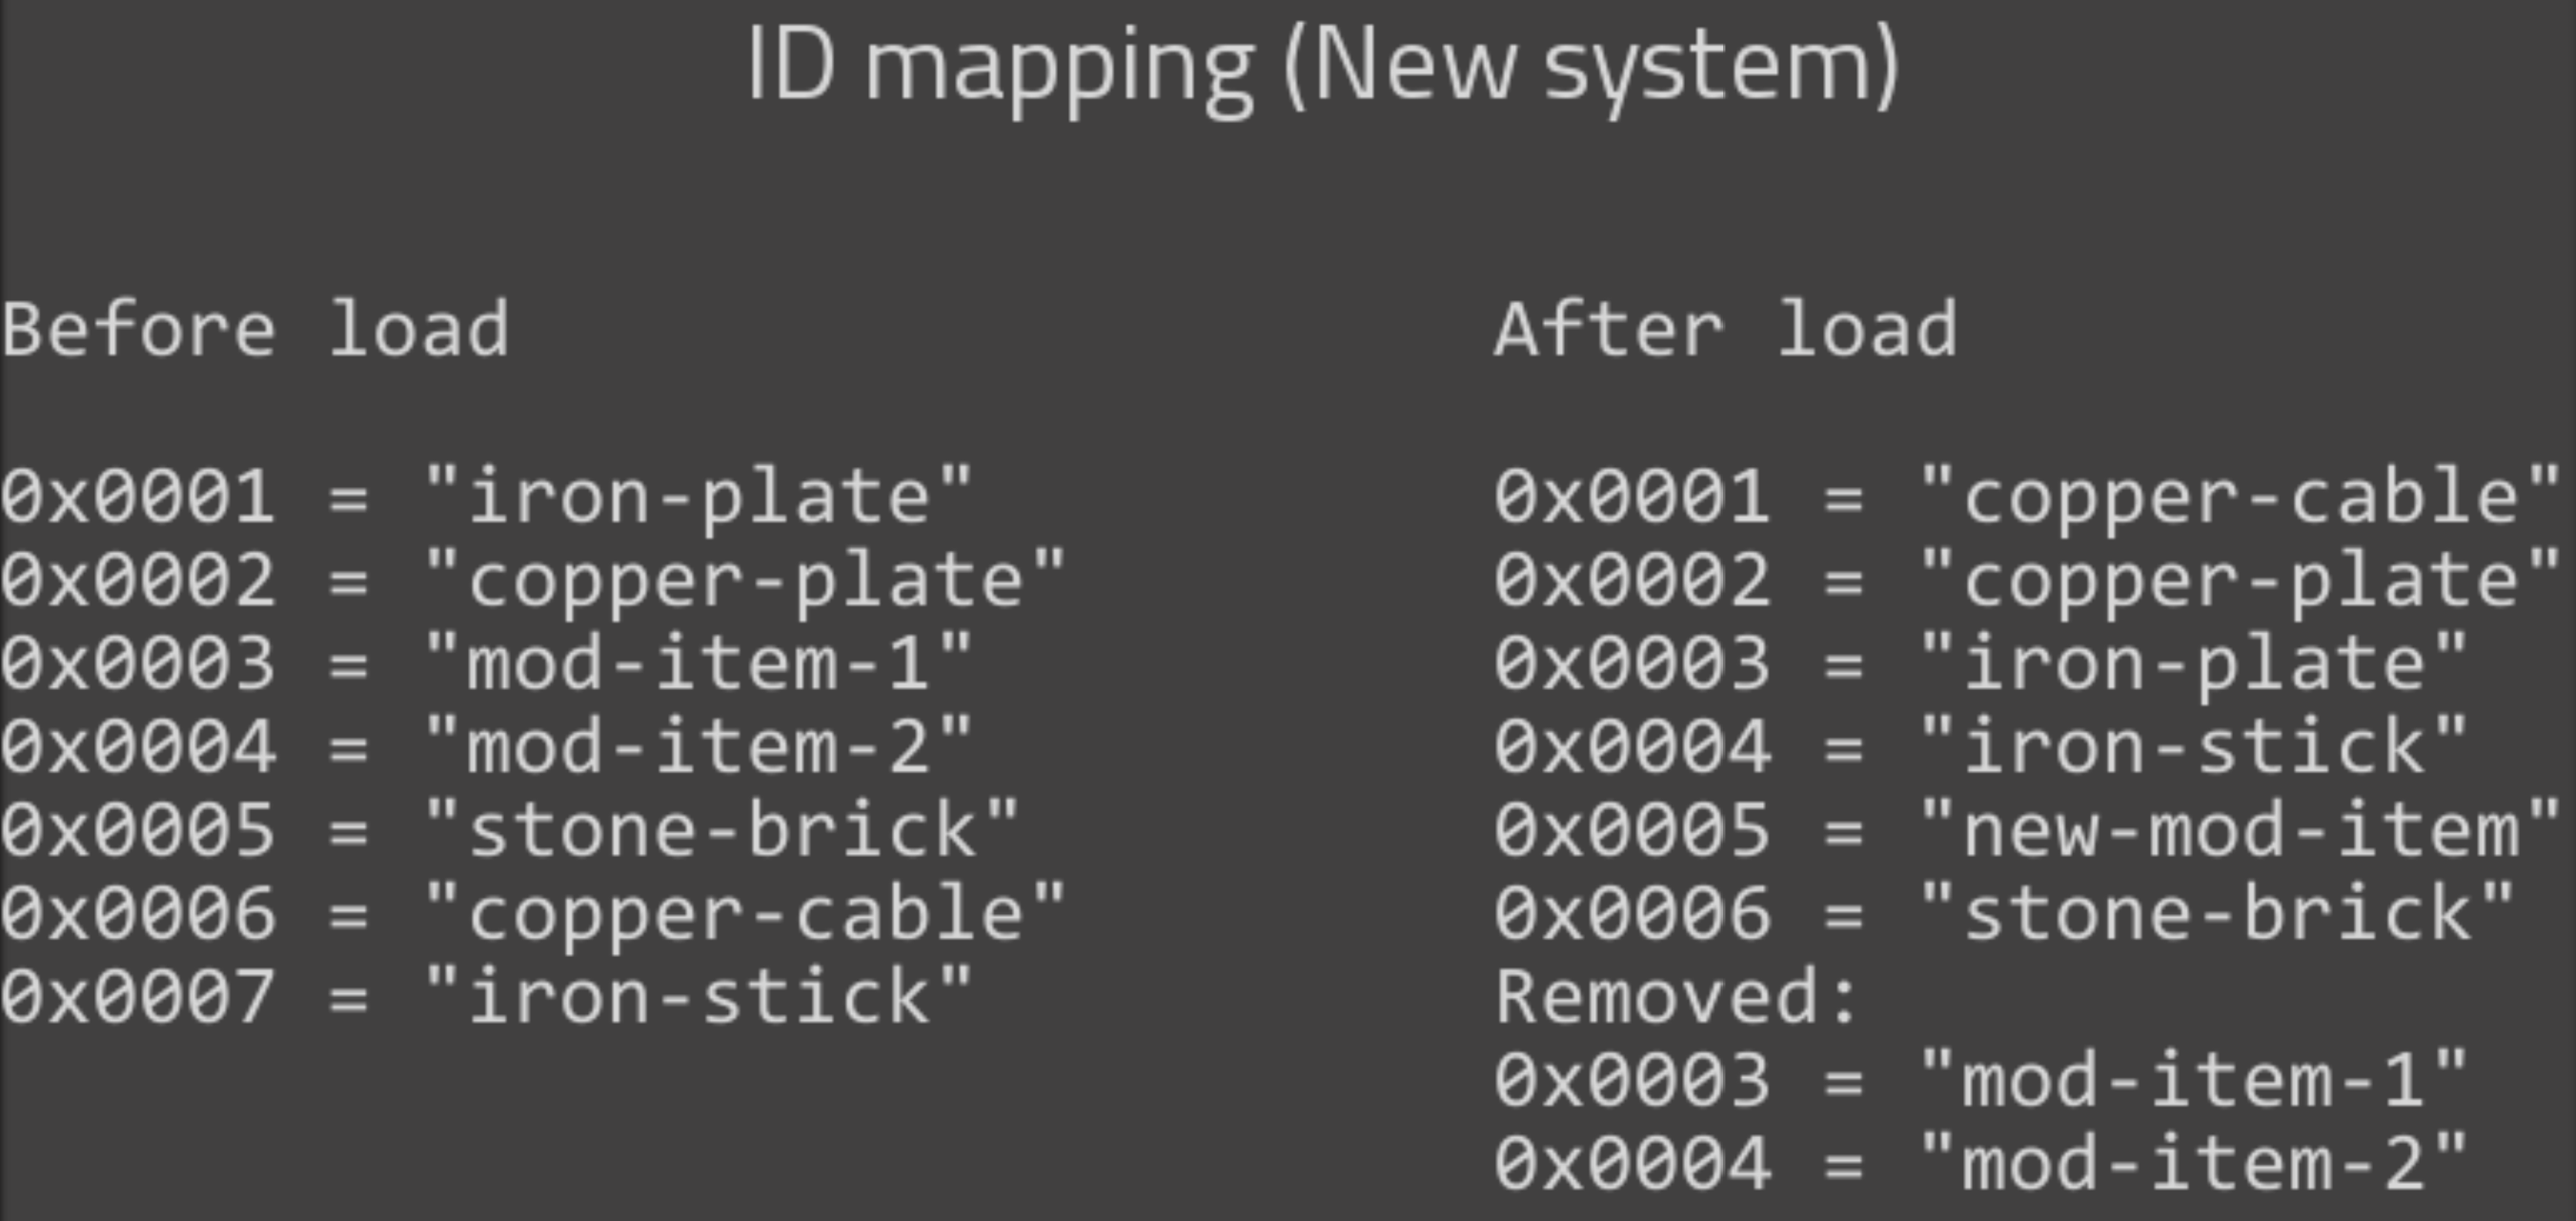
\includegraphics[width=0.9\textwidth]{images/id_mapping_factorio.png}
    \caption{Spielobjekte und deren Identifikationsnummer eines Spielstands\cite{factorioFridayFacts259}}
    \label{fig:factorioIdMapping}
\end{figure}

Als nächstes werden die angewandten Prototyp-Migrationen gesichert.\cite{factorioGithubSaveLoad} Ein Prototyp ist eine Vorlage für Maschinen, Rezepte und andere Spielkonzepte in der Factorio Game Engine.\cite{factorioPrototypesDocs}

Anschließend werden restliche Daten, die noch gespeichert werden müssen, gesichert und die SaveHelper-Liste wird abgearbeitet. Das SaveHelper-System wird verwendet, um weitere Speicherprozesse auszuführen, nachdem alles gespeichert wurde. Dafür muss ein SaveHelper erstellt werden, der dann durch das SaveHelper-System in eine Warteschlange von SaveHelpern hinzugefügt wird. Diese Warteschlange wird am Ende des Speicherprozesses abgearbeitet und von jedem SaveHelper wird die "save"-Funktion aufgerufen.\cite{factorioGithubSaveLoad}



\subsection{Ladevorgänge}
Der Ladeprozess für Factorio ist etwas komplizierter. Es gibt einige Dinge, die beachtet werden müssen, wie das Überprüfen der Map-Version und die Migration dieser auf andere Versionen. Außerdem muss überprüft werden, ob es bei den Mods Veränderungen gab. Factorio bietet Entwicklern an, Modifikationen des Spieles zu programmieren. Diese Modifikationen, auch "Mods" genannt, können zu einem Spielstand hinzugefügt werden. Deshalb muss bei jedem Laden des Spielstandes überprüft werden, ob Mods hinzugefügt, gelöscht oder verändert wurden. Worauf auch geachtet werden muss, ist, ob es beschädigte oder invalide Speicherdateien gibt.\cite{factorioFridayFacts270} 
Wie sieht dann der komplette Ladeprozess von Factorio aus, damit all diese Faktoren beachtet werden?

Der erste Schritt beim Laden eines Spielstandes ist, dass die Map-Version der zu ladenden Map mit der Version der Map, in die die Daten geladen werden sollen, verglichen werden muss. Falls die Versionen unterschiedlich sind, muss die zu ladende Map auf der Version der Map, in die geladen wird, migriert werden. Dabei muss beachtet werden, dass nicht jede Version von Factorio unterstützt wird. Manche Versionen können zu alt oder zu neu sein und können damit nicht verwendet werden.\cite{factorioGithubSaveLoad}

Als nächstes muss überprüft werden, ob die Mods, die für den zu ladenden Spielstand aktiv sind, oder die Mod-Einstellung sich geändert haben. Falls dies der Fall ist, müssen zusätzliche Vorgänge vorgenommen werden, nachdem die Daten geladen wurden. Dafür wird die Flag "prototype data changed" in der Lade-Klasse gesetzt.\cite{factorioGithubSaveLoad}

Bevor irgendwas geladen wird, was eine Identifikationsnummer benutzt, muss die ID-Mapping geladen werden. Ohne diesen Schritt weiß das Programm nicht, welches Spielobjekt mit welcher Identifikationsnummer gespeichert wurde und es könnte zu fehlerhaftes Laden des Spielstand führen. Außerdem wird über diesen Schritt dem Programm vermittelt, welche Spielobjekte sich verändert haben oder gelöscht wurden. Falls Mods die Identifikationsnummer von Spielobjekten zu anderen Identifikationsnummer ändern wollen, geschieht das auch direkt am Anfang.\cite{factorioGithubSaveLoad}

Nachdem die Identifikationsnummern erfolgreich geladen und gegebenenfalls modifiziert wurden, können die Standard-Map Daten geladen werden. Diese beinhalten Entitäten, Chunks, physikalische Kräfte und Züge.\cite{factorioGithubSaveLoad}

Wenn dieser Prozess abgeschlossen hat werden die LoadHelpers geladen. LoadHelpers arbeiten genau wie SaveHelpers, nur dass bei denen eine "load"-Funktion aufgerufen wird. Die SaveHelpers werden auch erst dann abgearbeitet, wenn die ganzen Daten geladen wurden. Die Reihenfolge der Prozesse der LoadHelpers muss genau gespiegelt zu der Reihenfolge der Prozesse der SaveHelpers ablaufen.\cite{factorioGithubSaveLoad}

Beim Ladeprozess gibt es Spielobjekte, die gelöscht werden müssen, aber dies kann erst passieren, wenn der Ladeprozess terminiert ist. Diese Spielobjekte können jetzt ohne Sicherheitsprobleme gelöscht werden. Außerdem werden jetzt noch Entitäten hinzugefügt, bei denen das Laden deren Daten fehlerhaft war. Dies muss jetzt geschehen, da beim Laden der Daten sich zum Beispiel Chunks verändern können, was zu Problemen bei manchen Entitäten führen kann. Wenn diese nochmal geladen werden, werden diese Probleme überschrieben und gelöst.\cite{factorioGithubSaveLoad}

Eine weitere Funktion, die die LoadHelpers besitzen, ist die "setup"-Funktion. Als nächsten Schritt wird von allen LoadHelpers diese Funktion aufgerufen. In der Setup-Funktion ist Logik, die nach der Load-Funktion und vor der Setup-Funktion der einzelnen Entitäten ausgeführt werden soll.\cite{factorioGithubSaveLoad}

Falls die "prototype data changed"-Flag gesetzt wurde, müssen die Daten zum Stromnetz noch einmal gelöscht und neu berechnet werden. Wenn die Flag gesetzt wurde, kann es sein, dass die Begrenzung von Entitäten sich verändert hat. Damit kann sich auch das Stromnetz, in dem sich eine Entität befindet, verändert haben, weshalb diese Daten in diesem Fall noch einmal neu berechnet werden.\cite{factorioGithubSaveLoad}

Als nächstes wird die Setup-Funktion aller Entitäten aufgerufen. Dabei werden als Erstes die Setup-Funktionen aller Transportbänder und danach die der restlichen Entitäten aufgerufen. Diese Reihenfolge ist wichtig, da die Logik des Zusammenführens der Entitäten mit den Transportbändern, die Entitäten durchführen, die keine Transportbänder sind. Dafür sollten alle Transportbänder schon fertig eingerichtet sein. Falls neue Entitäten beim Aufrufen der Setup-Funktionen entstehen, müssen auch bei diesen deren Setup-Funktion aufgerufen werden.\cite{factorioGithubSaveLoad}

Anschließend wird die Funktion "postLoadHook" aufgerufen. Diese geht nochmal über jede Oberfläche der Spielwelt und stellt die Liste der aktiven Entitäten wieder her. Da beim vorherigen Schritt neue Entitäten entstehen können, kann die "postLoadHook"-Funktion erst jetzt aufgerufen werden.\cite{factorioGithubSaveLoad} 

Als nächstes werden alle Tiles überprüft, da manche Veränderungen der Tiles beim Ladeprozess andere Tiles invalide machen können. Diese Tiles müssen gelöscht werden und auch alle Entitäten, die auf diesen liegen. Das Löschen von Entitäten ist jedoch erst dann möglich, wenn diese fertig eingerichtet wurden, also nach dem Aufruf der Setup-Funktion. Anschließend werden die Oberflächen- und Zug-Daten eingerichtet.\cite{factorioGithubSaveLoad}

Jetzt können die Veränderungen durchgeführt werden, die abgearbeitet werden müssen, wenn die "prototype data changed"-Flag gesetzt wurde. Dafür gibt es Entitäten, die mit "alarmed" markiert wurden. Diesen muss jetzt weitergegeben werden, dass alle die Entitäten fertig eingerichtet wurden und die Veränderungen beginnen können.\cite{factorioGithubSaveLoad}

Zum Schluss werden alle Dummy-Objekte gelöscht, letzte Setup-Funktionen aufgerufen und die Lua-Daten geladen und wiederherstellt. Dummy-Objekte werden in einer Liste während des Ladeprozesses gesammelt. Ein Objekt wird zu dieser Liste hinzugefügt, wenn dieses Objekt während des Ladevorgangs migriert oder gelöscht wurde. Die Liste der Dummy-Objekte wird dann am Ende abgearbeitet, damit die Objekte endgültig ohne Sicherheitsprobleme entfernt werden können.\cite{factorioGithubSaveLoad}

Wie zu sehen ist, ist der Ladeprozess von Factorio um einiges aufwendiger als der Speicherprozess. Der Ladeprozess besteht noch aus ein paar weiteren Schritten, diese sind aber für das Verständnis des gesamten Ladeprozesses nicht relevant. Was auch zu erkennen ist, ist, dass der Ladeprozess aus wiederholtem laden, einrichten, beheben von Problemen und neu berechnen besteht. Da stellt sich die Frage, ob dies effizient gelöst wurde, oder ob die teilweise wiederholten Schritte gekürzt werden können. Vermutlich gibt es zu viele Abhängigkeiten bei der Reihenfolge der einzelnen Prozesse, weshalb wenig Spielraum für Optimierung vorhanden ist.\todo{Ladezeiten lang in der Realität?}



\subsection{Fazit}
\dots
%--------------------------------------------------------------------------



%--------------------------------------------------------------------------
\section{Stardew Valley}
Stardew Valley ist ein Indie-Simulationsspiel, welches von Eric Barone, auch bekannt als ConcernedApe, im Jahr 2016 veröffentlicht wurde. Die Hauptaufgabe des Spiels ist es, eine Farm aufzubauen und diese zu pflegen. Dabei können Pflanzen angebaut, Tiere gezüchtet, Maschinen und vieles mehr aufgebaut werden. Außerhalb der Farm ist es auch möglich Minen zu entdecken, gegen Gegner zu kämpfen und an Seen und am Meer Fische zu fangen.\cite{steampoweredStardewValley} 

\todo{Save-Ordner auf Github und referenzieren}

\subsection{Daten}
Bei Stardew Valley gibt es viele verschiedene Arten von Daten. Einige Daten werden in vielen Teildaten aufgeteilt, wie zum Beispiel die Player- und Location-Daten. Außerdem gibt es noch viele weitere kleine Daten, zum Abspeichern des Spielstandes.

Die \textit{Player-Daten} bestehen aus Namen, wie der Spielername und Bauernhofname, Position des Spielers, der Quest-Log, die Items des Spielers, das Aussehen und noch vielen weiteren Daten, die den Zustand des Spielers abspeichern. Das Quest-Log ist eine Liste der Aufträgen, die der Spieler befolgen kann. Für jeden Auftrag gibt es einen Titel, eine Beschreibung, ein Ziel, die Belohnung die der Spieler bekommt für das umsetzen des Auftrages und noch weiteren kleinen Daten. Die Items werden als Liste gespeichert, wobei jeder Eintrag in der Liste ein Item ist, mit seinem Namen, Kategorie, Beschreibung, \ac{etc}. 

Die \textit{Locations} werden als Liste gesammelt. Die Listenelemente heißen \textit{GameLocation} und beinhalten eine Vielzahl an Informationen zu einer Ortschaft in dem Spiel. Es werden die Charaktere, Objekte, Terrain-Features, Gebäude, \ac{etc} in einer GameLocation gespeichert. Die einzelnen Charaktere bestehen aus einen Typen, Namen, deren Position und weitere relevante Daten, um Spielcharaktere abzuspeichern. Hier sind zum Beispiel Haustiere des Spielers oder \acp{npc} gespeichert. Die Objekte werden als Hashtabelle\footnote{Eine Hashtabelle ist eine Tabelle, die Schlüssel zu Werten zuordnet} gespeichert, wobei der Schlüssel ein zweidimensionaler Vektor ist, der die Position des Objektes angibt. Als Schlüsselwert werden alle Informationen zu dem Objekt aufgezählt, wie der Name, die Kategorie, der Preis, \ac{etc}. Die Terrain-Features werden auch als Hashtabelle gespeichert und beinhalte Informationen zu dem Gelände, wie zum zum Beispiel wo Bäume und Gräser platziert sind. Gebäude-Daten bestehen aus Informationen zu der Innenausstattung und den Charakteren in den Gebäuden.

Die restlichen Daten sind teilweise kleinere Daten, wie die Mailbox-Daten oder Statistiken. Bei der Mailbox wird nur die Email-Identifikationsnummer, während bei den Statistiken hauptsächlich Zahlen gespeichert werden. Statistiken wären zum Beispiel, wie viele Items ein Spieler gebaut hat oder wie viel Saatgut gesät wurde. Wie die Daten letztendlich aussehen wird in dem Abschnitt \ref{ssec:speicherformateStardew} genauer behandelt.

\subsection{Ordnerstruktur}
Die Ordnerstruktur von Stardew Valley ist recht schlicht gehalten, da die Anzahl der Daten im Vergleich zu den vorherigen Spielen klein sind. Für jede Spielwelt, die ein Spieler erstellt, gibt es einen eigenen Ordner. Der Name von diesem Ordner setzt sich aus dem Namen des Bauernhofs zusammen und eine Identifikationsnummer. In diesem Ordner sind dann vier Dateien. Die Dateien ohne der "\_old"-Endung haben den letzten Spielstand gespeichert und die mit dieser Endung den Spielstand davor. Dabei beinhalten die SaveGameInfo-Dateien Informationen, die im "Load Game"-Menü gebraucht werden. Die Daten zu einem Spielstand sind in der "<Bauernhof Name>\_<ID>"-Datei gespeichert, wobei der Name dieser Datei identisch zu dem des Ordners ist. Den kompletten Aufbau der Ordnerstruktur ist in der Abbildung \ref{lst:ordnerStrukturStardewValley} zu sehen. Die Daten in den Dateien werden im \ac{xml}-Format gespeichert, mehr dazu im Abschnitt \ref{ssec:speicherformateStardew}.\cite{stardewvalleywikiSaves}\cite{stardewvalleyFiles}

Wie zu sehen ist, gibt es bei Stardew Valley keine richtige Datenaufteilung, beim Speichern der Daten. Alle Informationen eines Spielstandes werden zusammen in einer Datei gesichert.

\begin{listing}[htp]
    \dirtree{%
    .1 <Bauernhof Name>\_<ID>.
        .2 \textcolor{blue}{SaveGameInfo}.
        .2 \textcolor{blue}{<Bauernhof Name>\_<ID>}.
        .2 \textcolor{blue}{SaveGameInfo\_old}.
        .2 \textcolor{blue}{<Bauernhof Name>\_<ID>\_old}.
    } 
    \caption{Ordnerstruktur einer Spielwelt in Stardew Valley}
    \label{lst:ordnerStrukturStardewValley}
\end{listing}

\subsection{Speicherformate} \label{ssec:speicherformateStardew}
Als Speicherformat wurde das \ac{xml}-Format verwendet. In den \ac{xml}-Codes aus \ref{lst:stardewvalleySaveGame} und \ref{lst:stardewvalleySaveGameInfo} ist zu sehen, wie die Daten aufgeschrieben werden. Bei der Hauptdatei zum Speichern des Spielstandes, werden die Daten in einem SaveGame-Objekt geschrieben. Bei der SaveGameInfo-Datei werden die Daten in einem Farmer-Objekt gesichert.\cite{stardewvalleywikiSaves}

\begin{listing}[htp]
    \begin{minted}[breaklines,frame=single]{xml} 
        <?xml version="1.0" encoding="utf-8"?>
        <SaveGame
          xmlns:xsi="http://www.w3.org/2001/XMLSchema-instance"
          xmlns:xsd="http://www.w3.org/2001/XMLSchema">
          <player>
            <name>Spielername</name>
            ...
            <Position>
              <X>123</X>
              <Y>456</Y>
            </Position>
            ...
            <questLog>
              <Quest>...</Quest>
              <Quest>...</Quest>
              ...
            <questLog>
            ...
            <items>
                <Item xsi:type="Axe">...</Item>
                <Item xsi:type="Pickaxe">...</Item>
                ...
            </items>
            ...
            <farmName>Bauernhofname</farmName>
            ...
            <shirt>1</shirt>
            <hair>2</hair>
            <skin>3</skin>
          <player>
          <locations>
            <GameLocation xsi:type="FarmHouse">...</GameLocation>
            <GameLocation xsi:type="Farm">...</GameLocation>
            ...
          </locations>
          ...
        </SaveGame>
    \end{minted}
    \caption{Hauptdatei zum Speichern des Spielstandes}
    \label{lst:stardewvalleySaveGame}
\end{listing}

\begin{listing}[htp]
    \begin{minted}{xml} 
        <?xml version="1.0" encoding="utf-8"?>
        <Farmer
          xmlns:xsi="http://www.w3.org/2001/XMLSchema-instance"
          xmlns:xsd="http://www.w3.org/2001/XMLSchema">
          <name>Spielername</name>
          ...
          <Position>
            <X>123</X>
            <Y>456</Y>
          </Position>
          ...
          <questLog>
            <Quest>...</Quest>
            <Quest>...</Quest>
            ...
          <questLog>
          ...
            <farmName>Bauernhofname</farmName>
          ...
          <shirt>1</shirt>
          <hair>2</hair>
          <skin>3</skin>
          ...
        </Farmer>
    \end{minted}
    \caption{SaveGameInfo Datei}
    \label{lst:stardewvalleySaveGameInfo}
\end{listing}

\subsection{Speichervorgänge}
Die Speichervorgänge von Stardew Valley sind sehr schlicht gehalten. In der Spielwelt gibt es einen Tag-Nacht-Zyklus. Sobald der Spieler in dem Spiel in einem Bett, oder der Spielcharakter automatisch um zwei Uhr nachts schlafen geht, wird der komplette Spielstand abgespeichert. Falls das Programm vorher terminiert, ist der Spielstand des aktuellen Tages im Spiel verloren gegangen.\cite{stardewvalleywikiSaves}

\subsection{Fazit}
\dots
